\documentclass[11pt]{scrreprt}
\usepackage[utf8]{inputenc}
\usepackage{graphicx}
\usepackage{listings} %插入代码
\usepackage{xcolor} %代码高亮
%\usepackage[demo]{graphicx}
\usepackage{caption}
\usepackage{tabularx}
\usepackage[labelformat=simple]{subcaption}

\renewcommand\thesubfigure{(\alph{subfigure})} % see subcaption doc

\lstset{numbers=left, %设置行号位置
	numberstyle=\tiny, %设置行号大小
	keywordstyle=\color{blue}, %设置关键字颜色
	commentstyle=\color[cmyk]{1,0,1,0}, %设置注释颜色
	frame=single, %设置边框格式
	escapeinside=``, %逃逸字符(1左面的键),用于显示中文
	breaklines, %自动折行
	extendedchars=false, %解决代码跨页时,章节标题,页眉等汉字不显示的问题
	xleftmargin=2em,xrightmargin=2em, aboveskip=1em, %设置边距
	tabsize=4, %设置tab空格数
	showspaces=false %不显示空格
}

\title{\textbf{Project 3 Report}}
\subtitle{CS325 Analysis of Algorithms, Summer 2015}
\author{\textsf{\textbf{Project Group 1}}\\
		\textsf{Tingzhi Li}\\
		\textsf{Nicholas Nelson}\\
		\textsf{Chunyang Zhang}}
\date{}

\begin{document}
\maketitle

\chapter{Transshipment Model}
\section{Part A}
The transshipment model is an extension of the transportation model. 
In addition to the standard transportation model, there are now 
intermediate transshipment points added between the sources (plants) 
and destinations (retailers). Items being shipped from a Plant 
($p_i$) must be shipped to a Warehouse ($w_j$) before being shipped 
to the Retailer ($r_k$). Each Plant will have an associated supply 
($s_i$) and each Retailer will have a demand ($d_k$). The number of 
plants is $n$, number of warehouses is $q$ and the number of 
retailers is $m$. The edges $(i,j)$ from plant ($p_i$) to warehouse 
($w_j$) have associated costs denoted $cp(j,k)$.

\subsection{i. Linear Formulation}

The objective function and constraints for this problem are as 
follows:

\begin{itemize}
	\item Minimize
[$10x_{1,1}+15x_{1,2}+11x_{2,1}+8x_{2,2}+13x_{3,1}+8x_{3,2}+9x_{3,3}+14x_{4,2}+8x_{4,3}+5y_{1,1}+6y_{1,2}+7y_{1,3}+10y_{1,4}+12y_{2,3}+8y_{2,4}+10y_{2,5}+14y_{2,6}+12y_{3,5}+12y_{3,6}+6y_{3,7}$] 
where $x_{i,j}$ represents number of refrigerators to be shipped 
from plant $i$ to warehouse $j$, and $y_{j,k}$ represents number of 
refrigerators to be shipped  from warehouse $j$ to retailer $k$.
	\item Supply constraints:
	\begin{enumerate}
		\item $x_{1,1} + x_{1,2} <= 150$
		\item $x_{2,1} + x_{2,2} <= 450$
		\item $x_{3,1} + x_{3,2} + x_{3,3} <= 250$
		\item $x_{4,2} + x_{4,3} <= 150$
	\end{enumerate}
	\item Retailer constraints:
	\begin{enumerate}
		\item $y_{1,1} >= 100$
		\item $y_{1,2} >= 150$
		\item $y_{1,3} + y_{2,3} >= 100$
		\item $y_{1,4} + y_{2,4} + y_{3,4} >= 200$
		\item $y_{2,5} + y_{3,5} >= 200$
		\item $y_{2,6} + y_{3,6} >= 150$
		\item $y_{3,7} >= 100$
	\end{enumerate}
	\item The number of refrigerators shipped into any individual 
		warehouse has to be equal to the number of refrigerators 
		shipped out from that warehouse, thus constrained by:
	\begin{enumerate}
		\item $x_{1,1} + x_{2,1} + x_{3,1} - y_{1,1} - y_{1,2} - y_{1,3} - y_{1,4} = 0$
		\item $x_{1,2} + x_{2,2} + x_{3,2} + x_{4,2} - y_{2,3} - y_{2,4} - y_{2,5} - y_{2,6} = 0$
		\item $x_{3,3} + x_{4,3} - y_{3,4} - y_{3,5} - y_{3,6} - y_{3,7} = 0$
	\end{enumerate}
\end{itemize}

\subsection{ii. Optimal Solution and Linear Program}

The optimal solution for this problem is as follows:\\

Objective value: 17100\\

\begin{tabular}{|c|c|c|c|c|c|c|c|c|c|}
	\hline variables & $x_{1,1}$   &  $x_{1,2}$ & $x_{2,1}$ & $x_{2,2}$ & $x_{3,1}$ & $x_{3,2}$ & $x_{3,3}$ & $x_{4,2}$ & $x_{4,3}$      \\
	\hline optimal value & 150  &  0 & 200 & 250 & 0 & 150 & 100 & 0 & 150            \\
	\hline
\end{tabular} \\

\begin{tabular}{|c|c|c|c|c|c|c|c|c|c|c|c|c|}
	\hline variables & $y_{1,1}$ & $y_{1,2}$ & $y_{1,3}$ & $y_{1,4}$ & $y_{2,3}$ & $y_{2,4}$ & $y_{2,5}$ & $y_{2,6}$ & $y_{3,4}$ & $y_{3,5}$ & $y_{3,6}$ & $y_{3,7}$  \\
	\hline optimal value & 	100 & 150 & 100 & 0 & 0 & 200 & 200 & 0 & 0 & 0 & 150 & 100 \\
	 \hline
\end{tabular} \\

Lindo Code

\begin{lstlisting}[language=c]
min 10x11+15x12+11x21+8x22+13x31+8x32+9x33+14x42+8x43+5y11+6y12+7y13+10y14+12y23+8y24+10y25+14y26+14y34+12y35+12y36+6y37
ST
	x11 + x12 <= 150
	x21 + x22 <= 450
	x31 + x32 + x33 <= 250
	x42 + x43 <= 150

	y11 >= 100
	y12 >= 150
	y13 + y23 >= 100
	y14 + y24 + y34 >= 200
	y25 + y35 >= 200
	y26 + y36 >= 150
	y37 >= 100

	x11 + x21 + x31 - y11 - y12 - y13 - y14 = 0
	x12 + x22 + x32 + x42 - y23 - y24 - y25 - y26 = 0
	x33 + x43 - y34 - y35 - y36 - y37 = 0
\end{lstlisting}

\subsection{iii. Optimal Shipping Routes/Minimum Costs}
The optimal shipping routes, based upon minimizing costs, are as follows: \\

\begin{tabular}{|c|c|}
	\hline From plants to warehouses & From warehouses to retailers \\
	\hline $x_{1,1} = 150$ & $y_{1,1} = 100$ \\
	\hline $x_{2,1} = 200$ &$y_{1,2} = 150$ \\
	\hline $x_{2,2} = 250$ &$y_{1,3} = 100$ \\
	\hline $x_{3,2} = 150$ &$y_{2,4} = 200$ \\
	\hline $x_{3,3} = 100$ & $y_{2,5} = 200$  \\
	\hline $x_{4,3} = 150$ & $y_{3,6} = 150$  \\
	\hline & $y_{3,7} = 100$ \\
	\hline
\end{tabular} \\

Minimum cost = \$17,100

\section{Part B}
Due to old infrastructure, warehouse 2 is going to close eliminating 
all of the associated routes. Therefore, all calculations as to the
optimal shipping route and minimized costs must be re-evaluated. The 
feasability of shipping all refrigerators to either warehouse 1 or 3
and then to the retailers without using warehouse 2 must also be
evaluated.

\subsection{Evaluation}
Without warehouse 2, there is no optimal solution to the transshipment 
model. It is not feasible to ship all refrigerators to either warehouse
1 or 3 and then to the retailers without using warehouse 2. Even if 
plants $p_3$ and $p_4$ shipped all refrigerators to warehouse $w_3$, 
the demands from $r_5$, $r_6$ and $r_7$ would not be met because
$p_3 + p_4 < r_5 + r_6 + r_7$.

\section{Part C}
Instead of closing warehouse 2, management has decided to keep a 
portion of it open but limit shipments to 100 refrigerators per week. 
The feasability of this model must be evaluated, and an optimal 
solution determined.

\subsection{Evaluation}
With warehouse 2 limited to 100 refrigerators per week, the model is
feasible. The optimal shipping routes, based upon minimizing costs, 
are as follows: \\

\begin{tabular}{|c|c|}
	\hline From plants to warehouses & From warehouses to retailers \\
	\hline $x_{1,1} = 150$ & $y_{1,1} = 100$ \\
	\hline $x_{2,1} = 350$ & $y_{1,2} = 150$ \\
	\hline $x_{2,2} = 100$ & $y_{1,3} = 100$  \\
	\hline $x_{3,3} = 250$ & $y_{1,4} = 150$  \\
	\hline $x_{4,3} = 150$ & $y_{2,4} = 50$  \\
	\hline 				  & $y_{2,5} = 50$ \\
	\hline 				  & $y_{3,5} = 150$ \\
	\hline 				  & $y_{3,6} = 150$ \\
	\hline 				  & $y_{3,7} = 100$ \\
	\hline
\end{tabular} \\

Minimum cost = \$18300

\section{Part D}
The generalized linear programming model for the transshipment problem 
can be expressed using the following formulation, objective function,
and constraints:\\

Objective function:
\begin{displaymath}
\min \left(\sum_{i=1}^{n} \sum_{j=1}^{q} cp(i,j)x_{ij} + \sum_{j=1}^{q} \sum_{k=1}^{m} cw(j,k)y_{jk}\right)
\end{displaymath}

$x_{ij}=0 \textrm{ if } cp(i,j) \textrm{ is not applicable, }$

$y_{jk}=0 \textrm{ if } cw(j,k) \textrm{ is not applicable,}$

where $x_{ij}$ represents the number of refrigerators to be shipped 
from plant $i$ to warehouse $j$ and $y_{jk}$ represents number of 
refrigerators to be shipped from warehouse $j$ to retailer $k$.\\

The constraints for this problem are as follows:

\begin{itemize}
	\item Supply constraints:
	\begin{displaymath}
	\sum_{j=1}^{q} x_{ij} \leq s_i 
	\qquad\textrm{where } i=1,2,\cdots,n
	\end{displaymath}
	\item Retailer constraints:
	\begin{displaymath}
	\sum_{j=1}^{q} y_{jk} \leq d_k 
	\qquad\textrm{where } k=1,2,\cdots,m
	\end{displaymath}
	\item The number of refrigerators shipped into any individual 
	warehouse has to be equal to the number of refrigerators 
	shipped out from that warehouse, thus constrained by:
	\begin{displaymath}
	\sum_{i=1}^{n} x_{ij} = \sum_{k=1}^{m} y_{jk} 
	\qquad\textrm{where } j=1,2,\cdots,q
	\end{displaymath}
\end{itemize}




\chapter{A Mixture Problem}

\section{Part A}
Veronica the owner of Very Veggie Vegeria is creating a new 
healthy salad that is low in calories but meets certain 
nutritional requirements. A salad is any combination of the 
following ingredients:\\

Tomato, Lettuce, Spinach, Carrot, Smoked Tofu, Sunflower Seeds, Chickpeas,
Oil\\

Each salad must contain:

\begin{itemize}
	\item At least 15 grams of protein
	\item At least 2 and at most 8 grams of fat
	\item At least 4 grams of carbohydrates
	\item At most 200 milligrams of sodium
	\item At least 40\% leafy greens by mass
\end{itemize}

The nutritional contents of these ingredients (per 100 grams)
and cost are:

\begin{figure}[!htbp]
	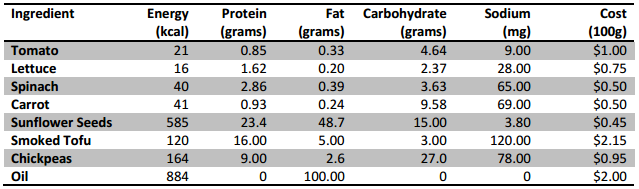
\includegraphics[width=1.0\textwidth]{nutritional.png}
\end{figure}

\subsection{i. Linear Formulation}
The objective function and constraints for this problem are as 
follows:

\begin{itemize}
	\item Minimize
[$210x_{1}+160x_{2}+400x_{3}+410x_{4}+1200x_{5}+5850x_{6}+1640x_{7}+8840x_{8}$]
where $x_{i}$ represents the weight (in 1000 gram/1 kgram units) for ingredient $i$.
	\item Supply constraints:
	\begin{enumerate}
		\item $x_{11} + x_{12} <= 150$
		\item $x_{21} + x_{22} <= 450$
		\item $x_{31} + x_{32} + x_{33} <= 250$
		\item $x_{42} + x_{43} <= 150$
	\end{enumerate}
	\item Retailer constraints:
	\begin{enumerate}
		\item $y_{11} >= 100$
		\item $y_{12} >= 150$
		\item $y_{13} + y_{23} >= 100$
		\item $y_{14} + y_{24} + y_{34} >= 200$
		\item $y_{25} + y_{35} >= 200$
		\item $y_{26} + y_{36} >= 150$
		\item $y_{37} >= 100$
	\end{enumerate}
	\item The number of refrigerators shipped into any individual 
		warehouse has to be equal to the number of refrigerators 
		shipped out from that warehouse, thus constrained by:
	\begin{enumerate}
		\item $x_{11} + x_{21} + x_{31} - y_{11} - y_{12} - y_{13} - y_{14} = 0$
		\item $x_{12} + x_{22} + x_{32} + x_{42} - y_{23} - y_{24} - y_{25} - y_{26} = 0$
		\item $x_{33} + x_{43} - y_{34} - y_{35} - y_{36} - y_{37} = 0$
	\end{enumerate}
\end{itemize}

\subsection{ii. Optimal Solution and Linear Program}
\subsection{iii. Cost of Low Calorie Salad}

\section{Part B}


\section{Part C}

\chapter{Shortest Path Problems}

\section{a}
\section{b}
\section{c}
\section{d}


\end{document} 
